% !Mode:: "TeX:UTF-8"
%%% Local Variables:
%%% mode: latex
%%% TeX-master: t
%%% End:

% 绪论和个人工作

\chapter{绪论}
\label{cha:intro}
近些年来,随着互联网的快速发展,人工智能和大数据技术的兴起和应用,网络数据、信息和知识大量增长。
传统的基于网页链接检索的信息存储、信息检索方式越来越难于进行查找学习知识,随着移动设备
的增加,人们对于信息检索、知识获取的要求也越来越高,面对各种数据信息,
人们查找检索知识的需求越来越迫切,越来越期望能更好更快的检索了解学习知识。
随之知识库构建、推理和应用变得流行起来,越来越多的大学、科研机构和商业公司开始构建大规模知识库,如Google Knowledge Graph\cite{Dong},NELL\cite{NELL-aaai15},YAGO\cite{Suchanek:2007:YCS:1242572.1242667},
Freebase\cite{Bollacker2008FreebaseAC},DBpedia\cite{Bizer:2009:DCP:1640541.1640848}等。
这些知识库基于自动和半自动的信息抽取、众包、专家领域内知识等进行构建,
把互联网、书籍、数据库等各处非结构化的文本中数据结构化、抽取构建知识库,
获得了大量的实体、关系和属性信息,能为人们提供的方便快捷的信息查询、检索、知识学习途径。
这类知识库的数据完整性、数据精确性和数据质量等衡量指标非常高,
已经有很多基于知识库的系统被成功用于商业领域,如谷歌搜索引擎\footnote{https://googleblog.blogspot.com/2012/05/introducing-knowledge-graph-things-not.html},
微软的必应搜索\footnote{https://blogs.bing.com/search/2013/03/21/understand-your-world-with-bing/}等。
除了这些通用领域的知识库之外,也有很多领域知识库被构建和应用,知识库也被用于生物学\cite{Dumontier:2014:BRL:2878453.2878554}、金融学、教育学等各个领域,一些较为成熟的问答系统、个人手机助手如Siri、Google Assistant、微软小冰等也将知识库集成其中。

图\ref{kb}是一个简单的知识库例子,常见的知识库可以用有向图进行逻辑上的可视化表示。
图中展示了实体、实体和实体之间关系,其中实体是描述现实中实际存在的事物、地点、人物、事件如:北京师范大学、北京等,关系是描述实体和实体之间存在的某种联系和特征,如北京师范大学和北京存在着位于的关系。除此之外,
一个知识库中的三元组还可以分为关系型三元组和实体属性三元组。关系三元组典型的例子如:北京师范大学,位于,北京。其中“北京师范大学”和“北京”是实体,
属性事实三元组如:北京,人口,2150万。
其中“北京”是实体,“2150万”是描述实体属性的属性值,“人口”是北京这类实体具有的一种属性类型。
通常关系型三元组用来描述实体和实体之间的联系,实体属性三元组描述实体的属性事实特征,这些不同类型的三元组共同构成一个完整的知识库。

\begin{figure}[H]
\begin{center}
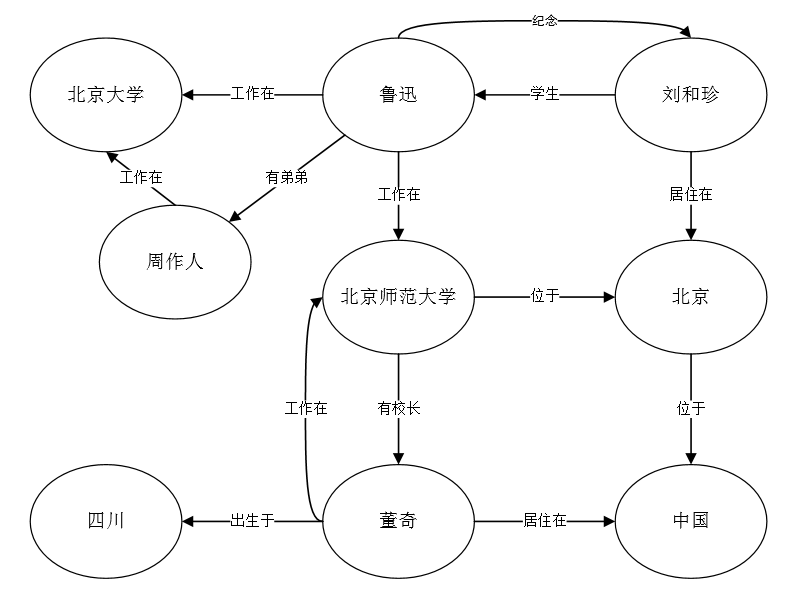
\includegraphics [width=0.5\textwidth]{kb.png}
\caption{一个知识库例子}
\label{kb}
\end{center}
\end{figure}

当前知识库相关的研究主要分为三个方面:(1)知识库的构建,各种基于互联网的、通用的、领域内的知识库构建。
(2)关系机器学习,基于已经构建好的知识库进行关系预测,知识库补全推理等。(3)知识库应用系统。如基于知识库的问答系统,
基于知识库的信息检索系统,生物、金融、教育等领域的本体知识库等。其中研究的热点之一就是知识库补全推理,即如何发掘知识库图结构中隐藏的关系。

当前存在的知识库系统如NELL、Knowledge Vault等,尽管已经包含了大量的实体、关系和属性,但这类知识库中很多实体和实体之间的关系任然是缺失的。例如,尽管知识库中存在很多三元组如:北师大,位于,北京;北京,位于,中国。但是当预测北师大是否位于中国时,通常计算机很难直接进行这类常识性的推理。如何构建一个辅助计算机进行常识推理系统,发现知识库中隐藏的实体和实体之间的关系,是知识库补全系统的重要任务之一。很多基于表示学习和基于符号逻辑的知识库补全算法被提出,这类算法都是基于知识库中现有的关系类型去预测知识库中未知的关系。但是在知识库中存在大量的属性事实型三元组未被使用,而这些属性事实三元组在进行关系预测时有很重要的作用,如:A,isMarriedTo,B,A,HasChild,C。当预测B是否是C的父母时,这些相关实体的年龄、性别等实体属性也很重要。

在构建知识库补全系统的过程中,基于符号逻辑的算法通常通过训练一个二分类的分类器来判断实体和实体之间是否具有某种关系。通常这个分类器的正例是通过抽取现有知识库中存在的三元组作为正例,或称之为正例三元组,而负例则是采用随机采样等方法生成负例三元组。通常在知识库补全系统中,每个正例三元组可以获得上万种不同的负例三元组,如何解决正负例三元组不均衡的问题,正确预测实体和实体之间的关系,也是知识库补全算法的一个重要优化方向。

\section{知识库构建}
在知识库构建过程中,数据完整性、数据精确性和数据质量是构建知识库的重要指标,
通常知识库可以由三元组组成。知识库的构建可以有多种方法:
(1)通过机器学习和自然语言处理技术自动抽取三元组\cite{Weikum2010FromIT}进行构建。
(2)半自动抽取的方法,通过从维基百科等网站的infobox基于规则模式抽取三元组。
(3)基于协同创作\cite{Vrandecic2014WikidataAF}的方法,通过众包的形式系统创建知识库。
(4)基于专家知识构建的领域内知识库,这些领域知识库有较高的专业性。

\subsection{YAGO知识库}
YAGO是一个从维基百科上抽取的、包含地理名词、WordNet\cite{Kasneci2008TheYA}等数据的知识库。
YAGO将WordNet的词汇定义与维基百科的分类体系进行了融合集成\cite{Suchanek2008YAGOAL},并集成了多种地理类型的数据,使得YAGO具有更加丰富的实体分类体系。YAGO还考虑了时间和空间知识\cite{Hoffart2011YAGO2EA},为很多知识条目增加了时间和空间维度的属性描述。目前,YAGO包含1.2亿条结合关系三元组和实体属性三元组的知识。YAGO也是IBM Watson\cite{Ferrucci2010BuildingWA}的后端知识库之一。
YAGO2\cite{Hoffart2013YAGO2AS}是YAGO的一个实例,当前YAGO2包括超过260万的实体和超过1.2亿的关系三元组知识,我们使用了其中实体的关系型三元组和属性型三元组共有4,484,914条、
37种关系型三元组的事实描述,同时有3,353,659条、35种属性性三元组的事实描述。

\subsection{Freebase知识库}
Freebase\cite{Bollacker2008FreebaseAC}是一个协同创作的知识库系统,内容通过用户添加,所有的条目采用结构化的形式,将结构分为三次:领域-类型-主题,其中,每一个条目叫做一个主题,每个主题包含不同的属性类型,一些同类型的主题组成一个类型,所有相关的类型构成一个领域。
这种通过协同创作方式创建了结构化的人类知识,截止2007年Freebase包含1.25亿条三元组,超过4000种类型和超过7000种属性知识。一些基于Freebase研究结构化知识的问答系统\cite{Yao2014InformationEO}\cite{Yao2015LeanQA},关注Freebase中的信息抽取和语义解析\cite{Yao2014FreebaseQI},也有一些研究关注Freebase中的实体消除歧义问题\cite{Zheng2012EntityDW}。

除了YAGO和Freebase知识库,也有很多重要的知识库如:Google Knowledge Graph,Wikidata,DBpedia等,这些通用的数据库都有着各自的特点和特色,表\ref{tab:addlabel-kb-list}展示了不同类型的知识库的实体、关系类型和三元组等数量,其中的M表示百万数量。本研究中的实验考虑到同时使用属性三元组和实体关系三元组,从而选择在YAGO和Freebase数据集中筛选属性特征较多的实体,
构建两个子数据集进行模型训练。

% Table generated by Excel2LaTeX from sheet '知识库'
\begin{table}[htbp]
  \centering
  \caption{不同知识库数据统计}
    \begin{tabular}{|l|l|r|l|}
    \hline
    知识库   & 实体数量  & \multicolumn{1}{l|}{关系类型数量} & 三元组数量 \\
    \hline
    Knowledge Graph & 570M  & 35000 & 18000M \\
    \hline
    YAGO2 & 9.8M  & 114   & 447M \\
    \hline
    DBpedia & 4.6M  & 1367  & 538M \\
    \hline
    Wikidata & 18M   & 1632  & 66M \\
    \hline
    Freebase & 40M   & 35000 & 637M \\
    \hline
    \end{tabular}%
  \label{tab:addlabel-kb-list}%
\end{table}%


\section{知识库应用}
知识库在通过自动、半自动的信息抽取、专家知识构建知识库后,有着各种各样广泛的应用,
并能辅助人们检索、学习通用知识;一些专家对领域内的知识进行有序化,规范化,
辅助人们去了解学习一个领域的专业知识。

知识库最广泛的应用是谷歌和微软等商业公司的信息检索系统,2014年谷歌提出的知识图谱\cite{Dong2014KnowledgeVA}就是结合FreeBase、Wikidata以及各种互联网数据进行信息抽取,
知识整合后的著名系统,谷歌也在其博客上讲述了如何将知识库应用在实际的检索中,
微软的Satori也是一个类似的知识库系统,被必应搜索广泛应用。其他搜索公司如百度、搜狗等公司都在知识库构建和信息检索领域有各自的应用,
对于每一个用户搜索的关键词,我们可以通过知识库系统来返回更丰富,更全面的信息。比如搜索一个企业法人的姓名,我们的智能搜索引擎可以返回与这个人相关的所有历史借款记录、联系人信息、行为特征等。另外我们通过可视化把复杂的信息以非常直观的方式呈现出来, 使得用户对于对隐藏信息的来龙去脉一目了然。

基于知识库的问答系统也有广泛的发展,2000年就有人提出基于知识的问答系统\cite{HERMJAKOB2000KnowledgeBasedQA},通过构架知识库完成问答。
也有很多方法基于知识库进行表示学习\cite{Yang2014JointRE},通过学习实体的低维度表示,学习知识库的实体和实体之间的关系,然后构建相关的知识库问答系统。
还有一些基于标签语义解析的方法,构建知识库问答系统\cite{Yih2016TheVO}。
一些论文\cite{Yu2017ImprovedNR}研究结合深度学习、关系抽取和问答系统,从而获得更好的知识库问答效果。
一些论文\cite{KeySun2016OpenKB}研究基于开放的知识库构建开放领域的问答系统,期望能基于百科知识进行问答系统构建。
也有基于知识库的系统通过结合智能计算\cite{Pandey2009KnowledgeAI},在医疗诊断领域获得一些突破。
也有一些研究结合了知识库和医疗图像信息\cite{Halpern2014EvaluationOC},对一些医疗疾病进行诊断治疗,期望能获得更好的治疗效果。

知识库在金融领域也可以有各种有效的应用。在进行金融风险检测时,
不一致性验证可以用来判断一个借款人的欺诈风险,这个跟交叉验证类似。比如借款人张三和借款人李四填写的是同一个公司电话,但张三填写的公司和李四填写的公司完全不一样,这就成了一个风险点,需要审核人员格外的注意。
除了贷前的风险控制,知识库也可以在贷后发挥其强大的作用。比如在贷后失联客户管理的问题上,知识库可以帮助我们挖掘出更多潜在的新的联系人,从而提高催收的成功率。

知识库也可以帮助我们分析用户和理解用户。通过结合多种数据源去分析实体之间的关系,从而对用户的行为有更好的理解。比如一个公司的市场经理用知识库来分析用户之间的关系,去发现一个组织的共同喜好,从而可以有针对性的对某一类人群制定营销策略。只有我们能更好的、更深入的理解用户的需求,我们才能更好地去做营销。

\section{知识库补全和推理}
虽然许多知识库的规模很大,但他们仍然是不完备的,如很多人的出生地点并未包含在知识库中,
一些演员是否出演过某些电影也是未知的。为了解决这个问题,很多知识库补全的方法被提出来,
这类方法基于知识库中已有的三元组预测新的三元组,如果将现有的知识库数据看做是多种关系构成的图,图的顶点是实体,图的边是实体对之间的关系,表\ref{tab:addlabel-relation}展示了YAGO和Freebase知识库中部分关系特征类型,知识库补全可以看成是图中关系的预测。
很多经典的知识库补全算法被提出,这些算法可以分为两类:基于逻辑符号推理的补全算法和基于表示学习的补全算法,
有时候也被称为基于图特征和基于隐藏特征的补全算法。

我们研究了常见的YAGO知识库,发现总共有四百多万实体关系数据被和三百多万属性事实的三元组。
其中的实体关系数据在以往经典的知识库补全算法中被广泛使用,而属性事实数据尽管大量存在,
却在知识库补全系统中并没有得到广泛应用,
同时实体属性数据类型单位差别很大,难以进行统一有效的处理,将这些实体属性特征作为知识库补全的特征也十分困难。
但可以预见在知识库关系预测中,实体属性特征会起着重要的作用,
如何将实体属性三元组有效用于知识库补全是本论文的关键点之一。

此外知识库中的图是稀疏的,每个存在的正例三元组实体对在训练模型中,
可能生成上百组负例三元组实体对,如何解决正负实体对不匹配的问题很关键,在正负实体对比例悬殊时,
关系预测中仅靠逻辑符号推理中的打分模型是不够的,在结果评价中并未考虑候选实体对的顺序对预测结果的影响,
也不关注候选实体的秩序关系,这也是知识库补全算法中需要解决的难点之一。

% Table generated by Excel2LaTeX from sheet 'Sheet1'
\begin{table}[htbp]
  \centering
  \caption{YAGO和Freebase知识库部分关系类型}
    \begin{tabular}{|l|r|}
    \hline
    YAGO关系类型 & \multicolumn{1}{l|}{Freebase关系类型} \\
    \hline
    isCitizenOf & \multicolumn{1}{l|}{/location/country/form\_of\_governme} \\
    \hline
    isAffiliatedTo & \multicolumn{1}{l|}{/tv/tv\_program/regular\_cast./tv/regular\_tv\_appearance/acto} \\
    \hline
    wasBornIn & \multicolumn{1}{l|}{/media\_common/netflix\_genre/titles} \\
    \hline
    playsFor & \multicolumn{1}{l|}{/award/award\_winner/awards\_won./award/award\_honor/award\_wi} \\
    \hline
    isLocatedIn & \multicolumn{1}{l|}{/soccer/football\_team/current\_roster./sports/sports\_team\_roster/position  } \\
    \hline
    influences & \multicolumn{1}{l|}{/sports/sports\_position/players./soccer/football\_roster\_position/t} \\
    \hline
    hasWonPrize & \multicolumn{1}{l|}{/film/film/starring./film/performance/acto} \\
    \hline
    dealsWith & \multicolumn{1}{l|}{/soccer/football\_team/current\_roster./soccer/football\_roster\_position/posi} \\
    \hline
    hasChild & \multicolumn{1}{l|}{/film/actor/film./film/performance} \\
    \hline
    graduatedFrom & \multicolumn{1}{l|}{/award/award\_nominated\_work/award\_nominations./award/award\_nomination/awar} \\
    \hline
    isMarriedTo & \multicolumn{1}{l|}{/award/award\_category/nominees./award/award\_nomination/nominated\_f} \\
    \hline
    worksAt & \multicolumn{1}{l|}{/award/award\_nominee/award\_nominations./award/award\_nomination/award\_nomin} \\
    \hline
    diedIn & \multicolumn{1}{l|}{/olympics/olympic\_sport/olympic\_games\_cont} \\
    \hline
    hasNeighbor & \multicolumn{1}{l|}{/music/performance\_role/regular\_performances./music/group\_membership/role } \\
    \hline
    happenedIn & \multicolumn{1}{l|}{/award/award\_category/winners./award/award\_honor/ceremony } \\
    \hline
    livesIn & \multicolumn{1}{l|}{/film/film/release\_date\_s./film/film\_regional\_release\_date/film\_release\_distribution\_mediu} \\
    \hline
    isPoliticianOf & \multicolumn{1}{l|}{/people/marriage\_union\_type/unions\_of\_this\_type./people/marriage/s} \\
    \hline
    participatedIn & \multicolumn{1}{l|}{/award/award\_winning\_work/awards\_won./award/award\_honor/award\_winn} \\
    \hline
    hasOfficialLanguage & \multicolumn{1}{l|}{/film/film/release\_date\_s./film/film\_regional\_release\_date/film\_release\_re} \\
    \hline
    owns  & \multicolumn{1}{l|}{/film/film/languag} \\
    \hline
    actedIn & \multicolumn{1}{l|}{/music/artist/genr} \\
    \hline
    \end{tabular}%
  \label{tab:addlabel-relation}%
\end{table}%


\section{本文工作重点和研究内容}

针对现有知识库补全技术不足,本研究将知识库中的关系路径特征和实体属性特征相结合,构建了一个更准确的知识库补全模型。首先,基于经典的路径排序模型抽取了关系路径特征;其次通过结合实体属性特征和关系路径特征,构建逻辑回归模型进行关系预测,从而进行知识库补全。
除此之外,本研究提供一种基于学习排序算法的知识库补全技术,
我们通过计算候选头实体和尾实体在关系预测中的位置排序,通过优化排序损失函数MAP来保证训练误差最小,
从而获得最优的关系预测结果,并选择合适的模型评价指标来评估改进我们的预测结果。

本研究的工作重点有三点:(1)特征计算,基于随机游走抽取关系路径特征,获得实体和实体之间有表达力的知识库补全路径,基于特征工程转化实体属性特征,将关系路径和实体属性路径结合,组合构建具有表达里的实体属性和关系路径特征,进而获得更加稳定,更加具有泛化能力的知识库补全特征。(2)提出了基于排序的知识库补全算法,将知识库补全算法从优化二分类模型改进为优化一组相关实体对排序的顺序问题,通过构建pairwise模型,进一步提升模型的预测能力。(3)探索基于深度神经网络的知识库补全算法,结合wide \& deep模型,将基于深度神经网络的排序算法用于知识库补全技术中,从而进一步提高模型的特征组合能力和模型泛化能力。

本研究的工作难点也较多:(1)实体属性特征的复杂性较大。在表\ref{tab:addlabel-attr}中,我们展示了YAGO和Freebase知识库中部分实体的属性特征。以YAGO知识库为例,
我们可以发现,常见的属性特征信息可以不仅仅有数量类型的如:hasNumberOfPeople、hasArea等,也有日期类型的特征信息如:wasCreatedOnDate、wasBornOnDate,也有比值型的实体属性特征如:hasInflation、hasUnemployment等。如何整合这些不同类型的特征信息,如何将属性特征和实体关系特征进行组合,都是本研究的重点和难点工作之一。(2)在知识库补全系统中,一个正例三元组通常可以配对成百条负例三元组,这种正负例三元组极其不平衡的问题通常需要构建合理的模型进行算法优化。如何构建合理有效的模型,优化知识库补全模型,是本研究的另一个难点之一。在基于表示学习的知识库补全算法中,不同的模型有不同的目标函数,通过机器学习优化算法,学习不同实体、关系的低维度表示向量。对于基于符号逻辑的知识库补全算法来说,常见的知识库补全算法如路径排序和子图特征抽取算法都是采用二分类模型进行知识库补全算法模型构建。如路径排序算法中,通常采用逻辑回归算法或者支持向量机回归,学习实体和实体之间具有某种关系的值。这种算法通常可以看做一种基于pointwise的知识库补全算法,然而,在一个知识库补全系统中,一组正负例实体对也可以当做一个整体进行优化,构建pairwise的知识库补全算法,进行模型优化,从而解决正负例实体对极其不平衡的问题。



% Table generated by Excel2LaTeX from sheet 'Sheet1'
\begin{table}[htbp]
  \centering
  \caption{YAGO和Freebase知识库中的部分实体属性特征}
    \begin{tabular}{|l|l|}
    \hline
    YAGO实体属性特征  & FB15K实体属性特征 \\
    \hline
    hasNumberOfPeople  & /tv/tv\_program/air\_date\_of\_first\_episode \\
    \hline
    hasArea  & /user/jg/default\_domain/olympic\_games/closing\_date \\
    \hline
    wasCreatedOnDate  & /user/jg/default\_domain/olympic\_games/opening\_date \\
    \hline
    hasLongitude  & /time/event/start\_date \\
    \hline
    hasPopulationDensity  & /time/event/end\_date \\
    \hline
    hasLatitude  & /user/maxim75/default\_domain/dbpedia\_import/geocode\_checked \\
    \hline
    wasBornOnDate  & /tv/tv\_program/air\_date\_of\_final\_episode \\
    \hline
    hasHeight  & /award/award\_category/date\_discontinued 16 \\
    \hline
    wasDestroyedOnDate  & /user/ktrueman/default\_domain/international\_organization/founded \\
    \hline
    diedOnDate  & /base/usnris/nris\_listing/significant\_year \\
    \hline
    hasLength  & /sports/pro\_athlete/career\_start \\
    \hline
    happenedOnDate  & /tennis/tennis\_player/year\_turned\_pro \\
    \hline
    hasUnemployment  & /royalty/order\_of\_chivalry/date\_founded 21 \\
    \hline
    hasEconomicGrowth  & /business/defunct\_company/ceased\_operations \\
    \hline
    hasRevenue  & /government/legislative\_session/date\_began \\
    \hline
    hasGini  & /government/legislative\_session/date\_ended \\
    \hline
    hasExpenses  & /music/artist/active\_start \\
    \hline
    hasInflation  & /people/deceased\_person/date\_of\_cremation \\
    \hline
    hasGDP  & /base/cdnpolitics/legislative\_assembly/founded \\
    \hline
    hasImport  & /royalty/royal\_line/ruled\_to \\
    \hline
    hasExport  & /royalty/royal\_line/ruled\_from \\
    \hline
    hasPoverty  & /music/artist/active\_end \\
    \hline
    hasBudget  & /sports/pro\_athlete/career\_end \\
    \hline
    hasWeight  & /base/lewisandclark/places\_eastward/from \\
    \hline
    hasDuration  & /base/yalebase/secret\_society/founded \\
    \hline
    \end{tabular}%
  \label{tab:addlabel-attr}%
\end{table}%




